\Needspace{12\baselineskip}
\originalchapter{数值复核与测量记录}
\originalsection{幅度阻尼恢复}
\par\noindent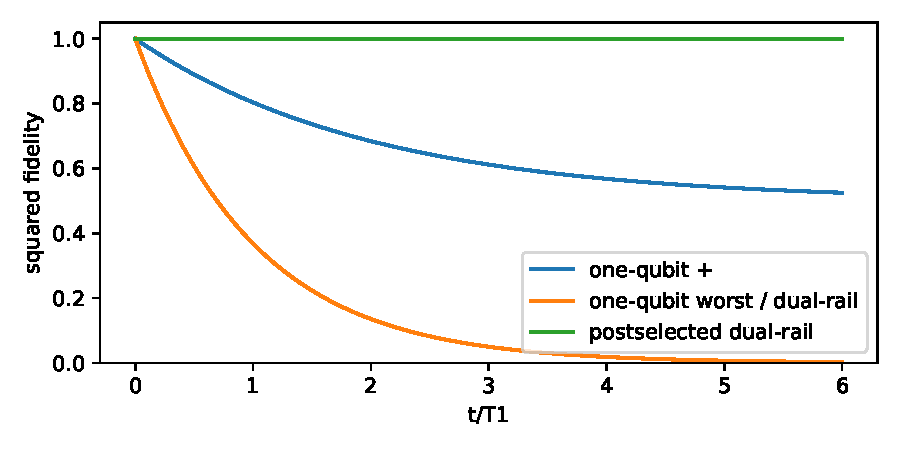
\includegraphics[width=.82\linewidth]{figures/amplitude-fidelities.pdf}\par
前图明确画$G=F^2$, 是PS1 P3根保真度的平方对照. 原题答案$F_+=\sqrt{(1+\e^{-t/(2T_1)})/2}$, $F_{\min}=F_{\rm dual}=\e^{-t/(2T_1)}$. 双轨后选择曲线必须同时读其成功概率$\exp(-t/T_1)$, 不表示确定性完美恢复.
\par\noindent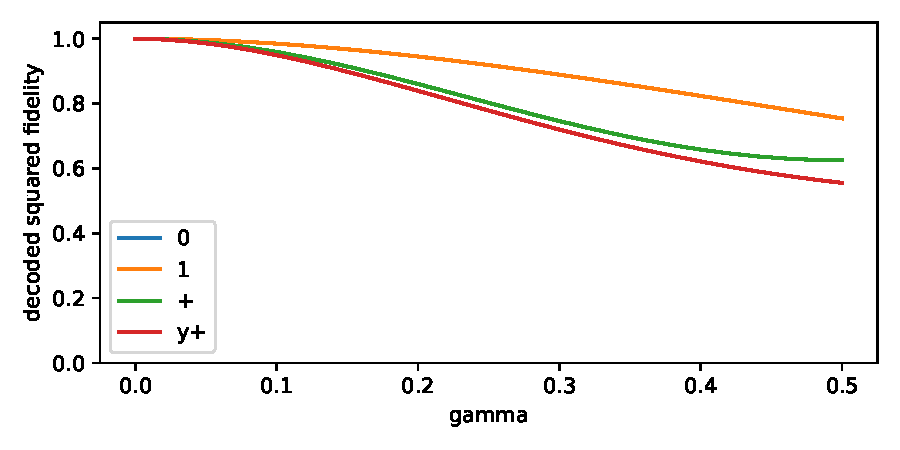
\includegraphics[width=.82\linewidth]{figures/shor-amplitude.pdf}\par
九位图使用作业一中明确的256综合征标准恢复, 对$0,1,+,y_+$四个输入直接求有限Kraus和. 完整逻辑信道的保迹误差与恢复基正交误差由脚本核验; 四个曲线不是对全部输入的最坏情形证明. 通用输入的精确表达在PS1 P3(f).

\originalsection{相位后验与反馈}
\par\noindent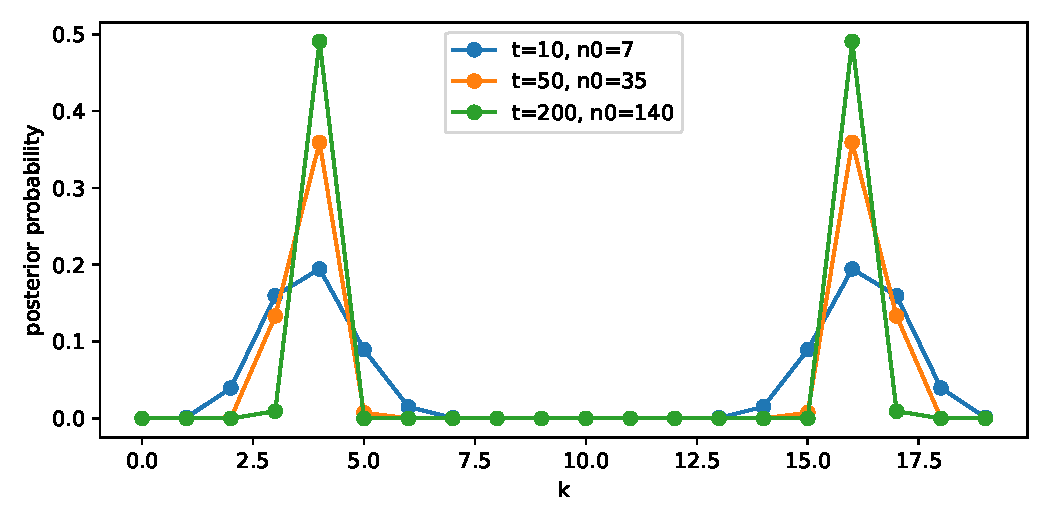
\includegraphics[width=.86\linewidth]{figures/phase-posteriors.pdf}\par
$n_0\simeq0.7t$, 后验按20个离散本征标签精确归一; 不使用原题错误的常数分母. 对称两峰说明仅cos概率不能分开$k,r-k$.
\par\noindent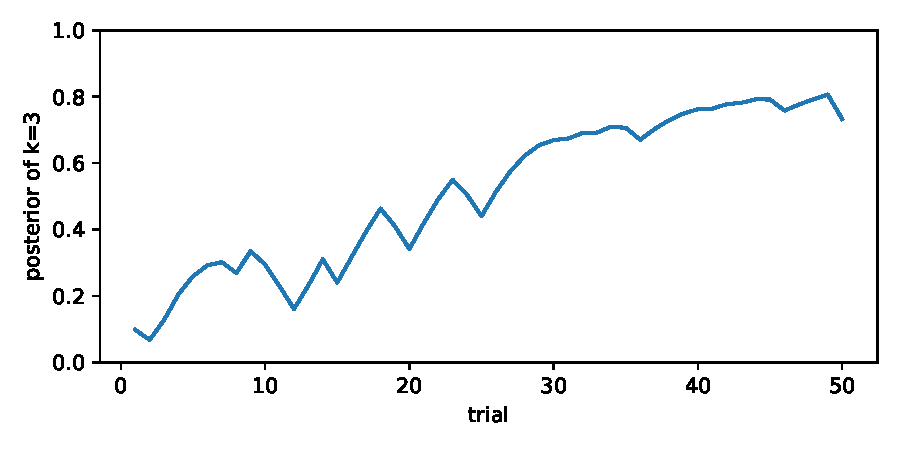
\includegraphics[width=.8\linewidth]{figures/phase-feedback.pdf}\par
反馈试验取真标签$k=3$, 随机种子143, 每步在200点相位网格最大化预期互信息再Bayes更新. 所有观测与相位值保存在\texttt{qa/feedback-record.json}; 不用单个成功试验宣称全局最优估计.

\originalsection{有限矩阵检查}
Fredkin的六个Pauli生成像与原8乘8矩阵逐项共轭核对, 残差低于$10^{-12}$. 相位匹配搜索检查$N=4,10,100,143,1024$均达到双精度容差内的成功率1. 典型串数以整数精确计算, 结果为
\[K=244260289238065954136071864320.\]
 需98位, 典型概率约0.618575. 这些有限实例验证不代替前面的一般证明.
